\documentclass{beamer}
\usepackage{textcomp}
\usepackage[utf8]{inputenc}
\usepackage{adjustbox}


\setbeamerfont{footnote}{size=\tiny}
\usetheme{Boadilla}
\usecolortheme{seagull}

\usepackage{fancyvrb}
\newenvironment{myverb}{% Verbatim shrinked
 \VerbatimEnvironment
 \begin{adjustbox}{max width=\linewidth}
 \begin{BVerbatim}
  }{
  \end{BVerbatim}
 \end{adjustbox}
}
\title{ATAC-Seq pipelines}
\author{\href{mailto:os@jetbrains.com}{Oleg Shpynov}}
\institute{JetBrains Biolabs}

\date{\today}

\begin{document}

\begin{frame}
  \titlepage
\end{frame}

\begin{frame}{Agenda}
\begin{itemize}
	\item ATAC
	\item Who is who?
	\item ATAC vs FAIRE
	\item Pipelines
\end{itemize}
\end{frame}

\begin{frame}{ATAC}
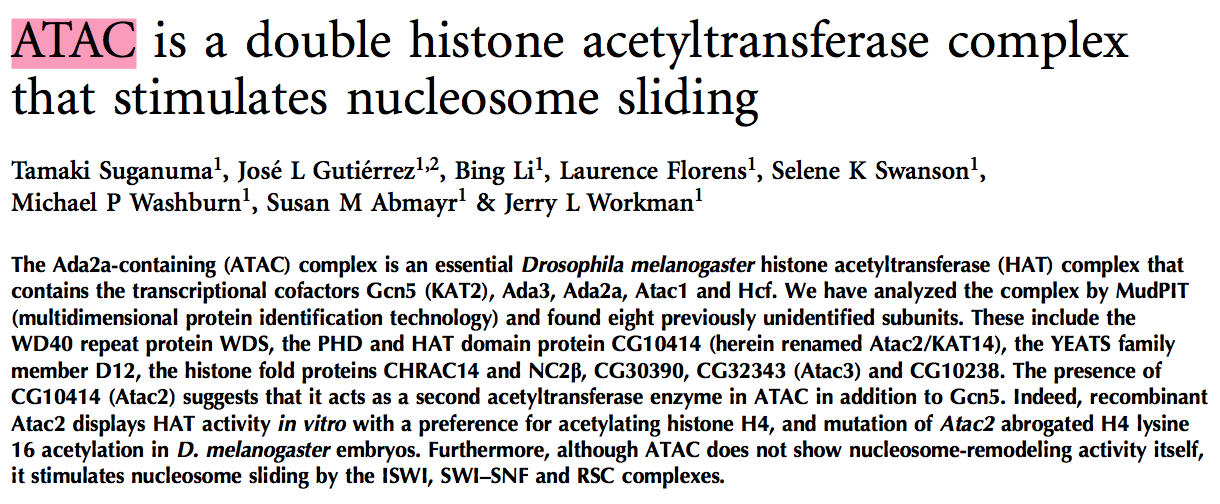
\includegraphics[width=\linewidth]{wrong_atac.png}\\
Be careful!
\end{frame}

\begin{frame}
\begin{block}{ATAC-Seq}
Assay for Transposase-Accessible Chromatin with high-throughput sequencing (ATAC-seq) is a method for mapping chromatin accessibility genome-wide. 
\end{block}
\end{frame}

\begin{frame}{High resolution mapping}
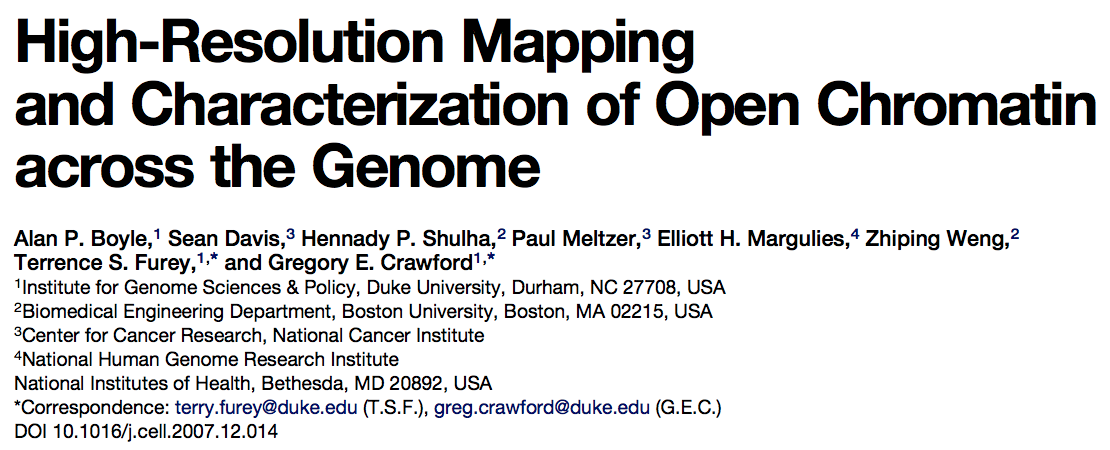
\includegraphics[width=\linewidth]{high_res_mapping.png}\footnote{650+ cited}\\
\textit{In addition, and unexpectedly, our analyses have uncovered detailed features of nucleosome structure.}
\end{frame}

\begin{frame}{DNAse I}
\centering{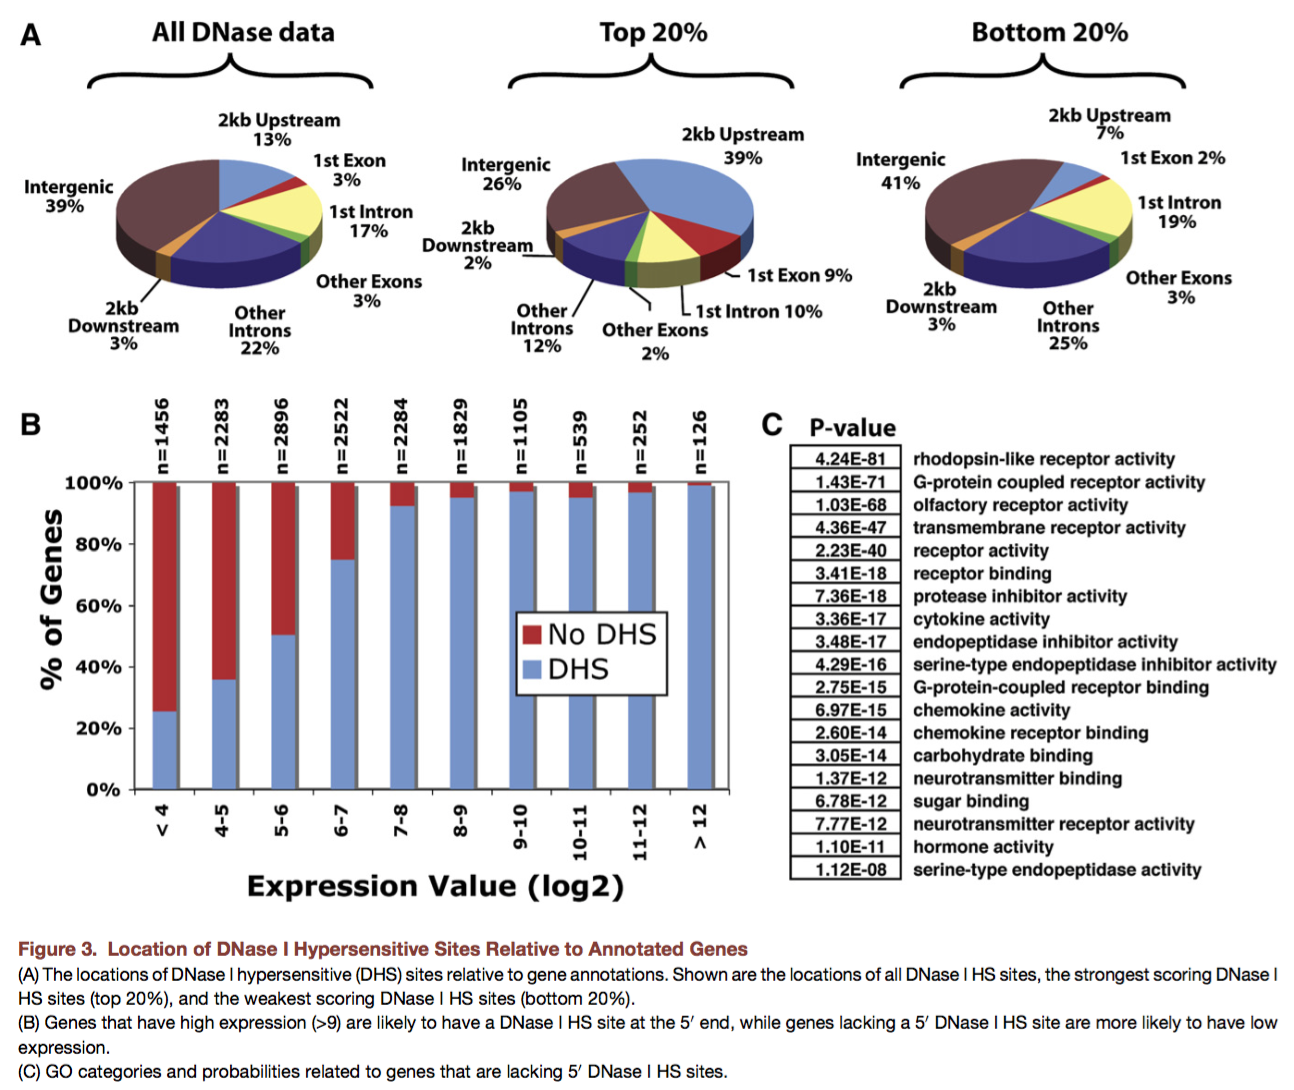
\includegraphics[height=0.85\paperheight]{dnase.png}}
\end{frame}

\begin{frame}{MNAse}
\centering{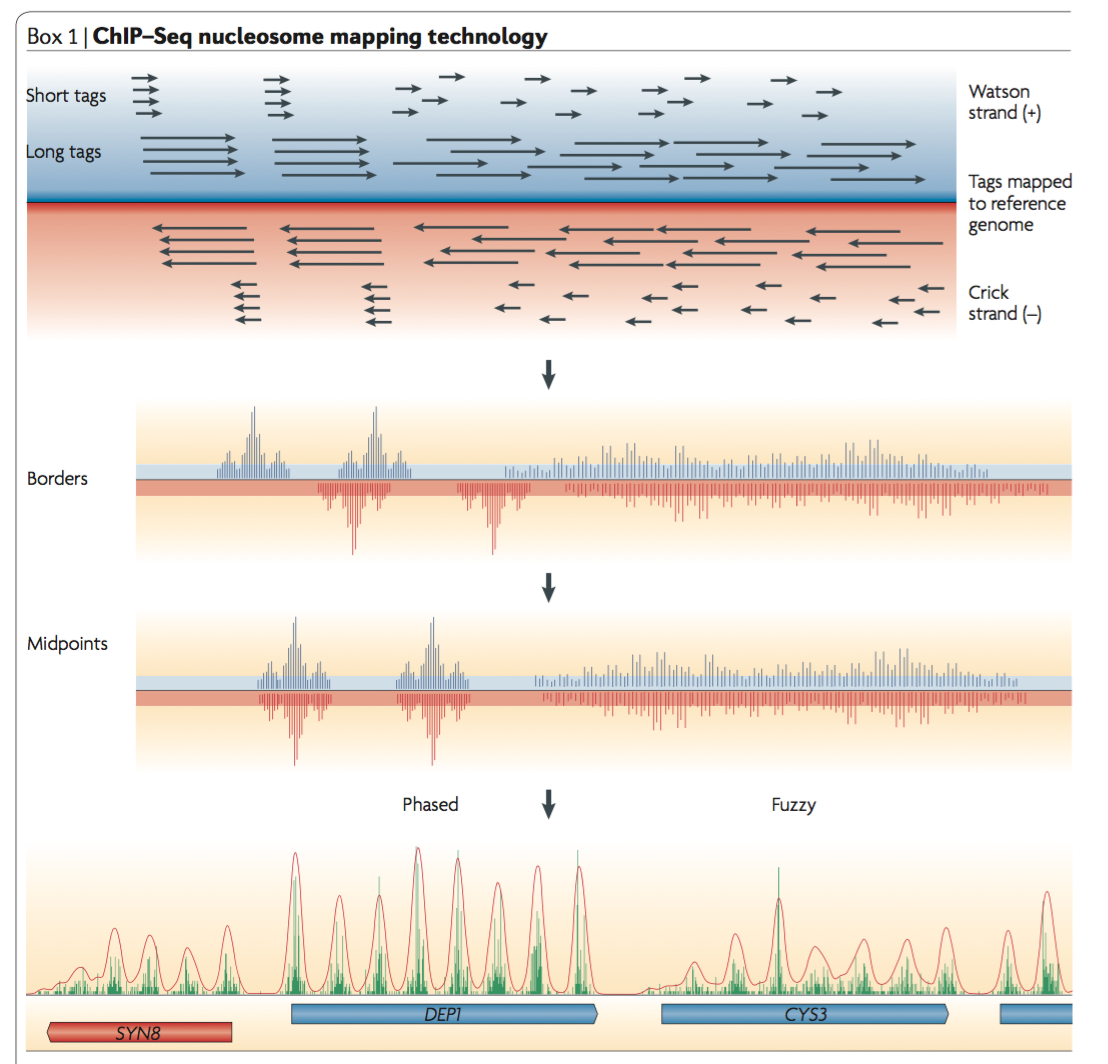
\includegraphics[height=0.85\paperheight]{mnase_mapping.png}\footnote{\url{http://www.nature.com/nrg/journal/v10/n3/full/nrg2522.html}}}
\end{frame}

\begin{frame}{Who is who?}
\centering{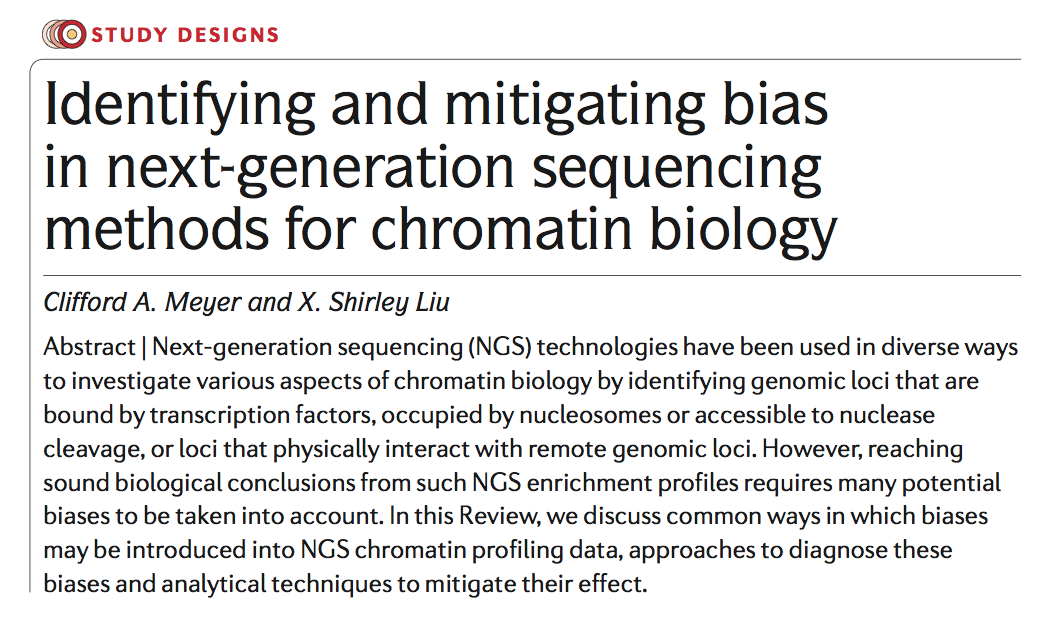
\includegraphics[width=\linewidth]{bias.png}}
\end{frame}

\begin{frame}
\centering{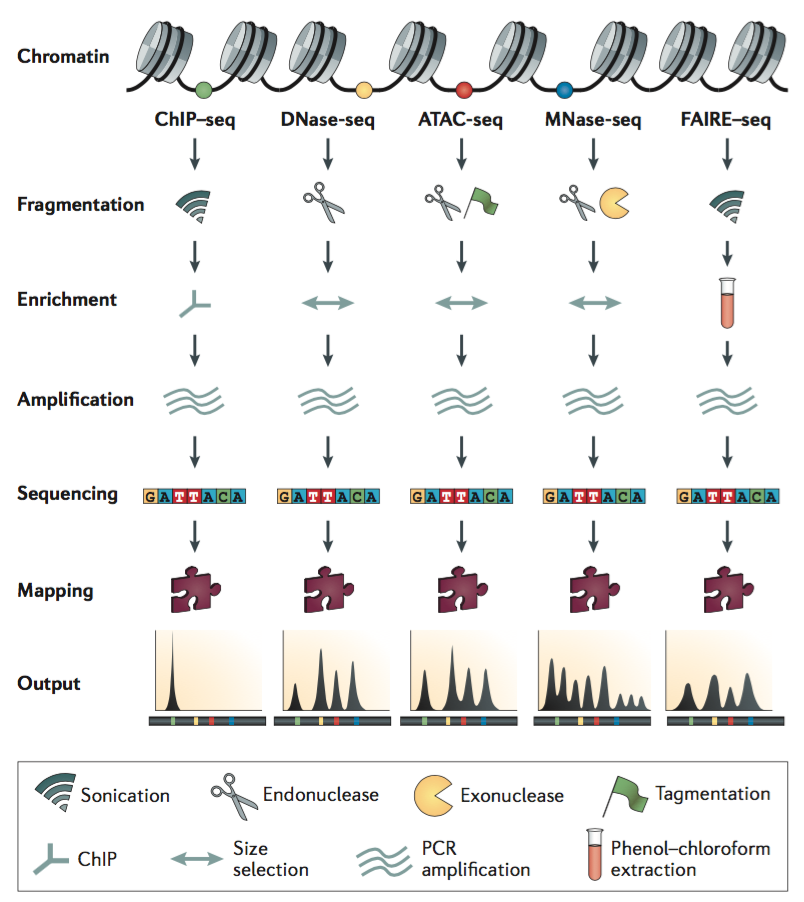
\includegraphics[height=0.85\paperheight]{whoiswho.png}}
\end{frame}

\begin{frame}{Bias, Bias, Bias, ...}
\begin{itemize}
\item Chromatin fragmentation and size selection: sonication, enzymatic cleavage. 
\item Controls for enzymatic cleavage assays. \\
\small{Genomic assays that are based on the selection of fragments produced from enzymatic DNA cleavage — including ATAC- seq, DNase-seq and MNase-seq — may be influenced by the tendency of the enzyme to cleave some DNA sequences more efficiently than others.}
\item Identifying Bias. \\
\small{The \textbf{ChiLin} quality control pipeline is a good starting point for understanding the quality and bias characteristics of ChIP–seq, DNase-seq and ATAC-seq samples. }
\end{itemize}
Summary: ATAC-seq requires fewer cells and less experimental calibration, but bias characteristics are not as well
understood as those of DNase-seq.\footnote{\url{http://www.ncbi.nlm.nih.gov/pubmed/24317252}}
\end{frame}

\begin{frame}{ChiLin}
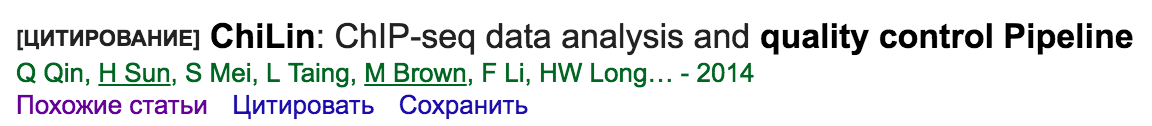
\includegraphics[width=\linewidth]{chilin.png}\\
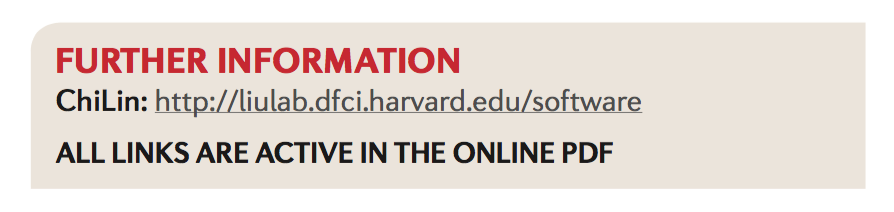
\includegraphics[width=\linewidth]{chilin404.png}\footnote{Correct url: \url{http://cistrome.org/chilin/}}\\
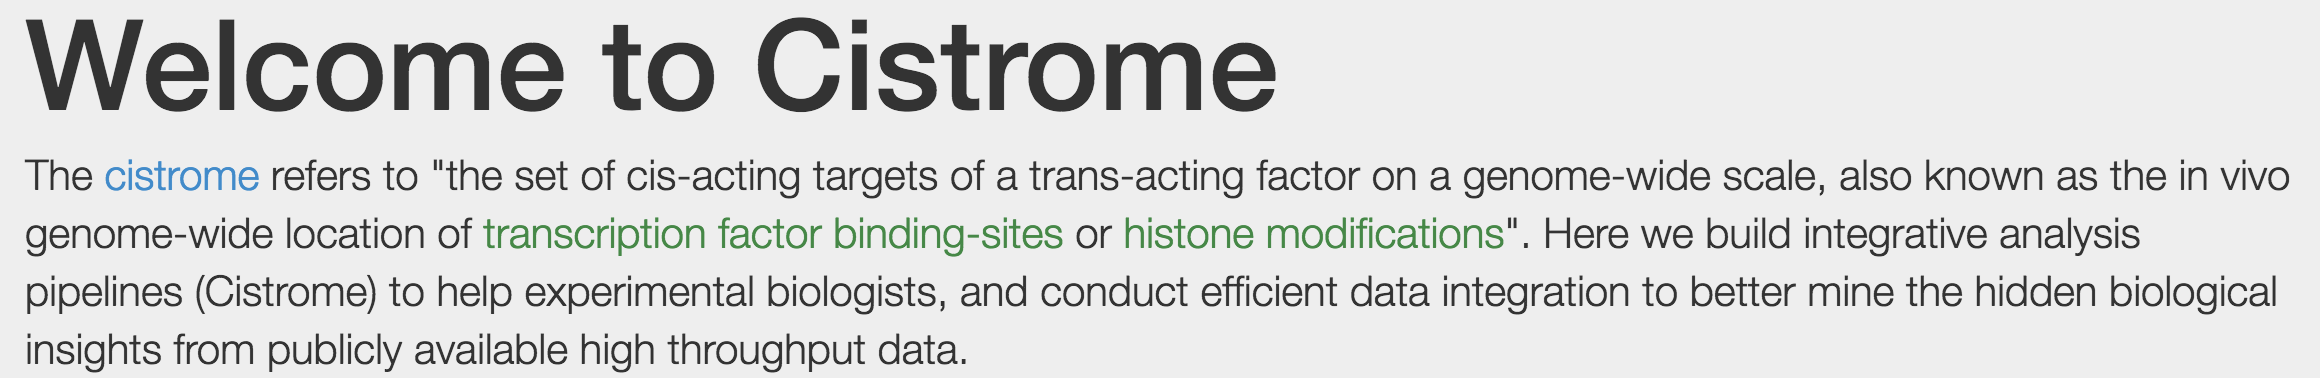
\includegraphics[width=\linewidth]{cistrome.png}\footnote{\url{http://cistrome.org/Cistrome/Cistrome_Project.html}}
\end{frame}

\begin{frame}{ATAC-Seq}
Paper 2014:\\
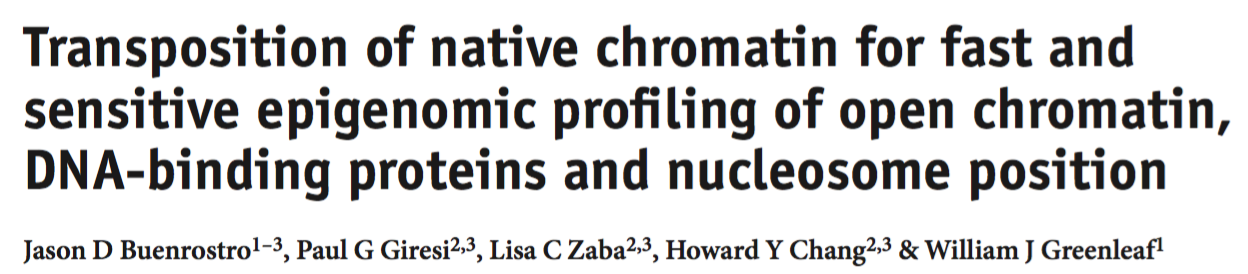
\includegraphics[width=\linewidth]{atac.png}\\
Protocol for humans 2015:\\
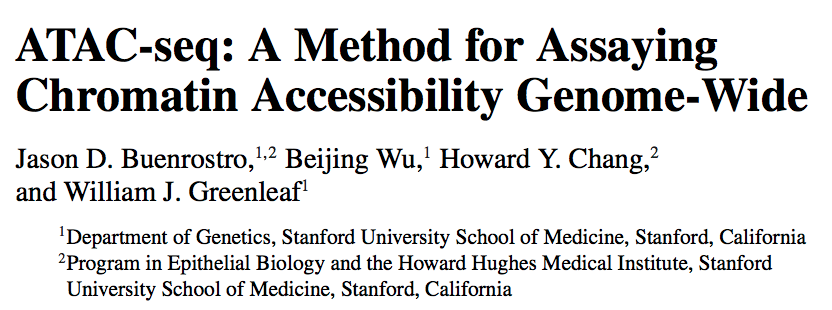
\includegraphics[width=\linewidth]{atac_protocol.png}\\
\end{frame}

\begin{frame}{Motivation}
MNase-seq, ChIP-seq, and DNase-seq in particular have proven to be information-rich, genome-wide analysis methods for understanding this epigenetic structure, providing information on transcription factor binding, the positions of modified and canonical nucleosomes, and chromatin accessibility...\\
However, \textbf{tens to hundreds of millions} of cells as input material are necessary.\footnote{1-50mln for GM12878 in paper 2014}\\

\begin{itemize}
\item Average over and ‘drown out’ heterogeneity in cellular populations
\item Cells must often be grown ex vivo to obtain sufficient material
\item No ‘personal epigenomes’ on diagnostic timescales
\end{itemize}
\end{frame}

\begin{frame}{Tagmentation, material, time}
\centering{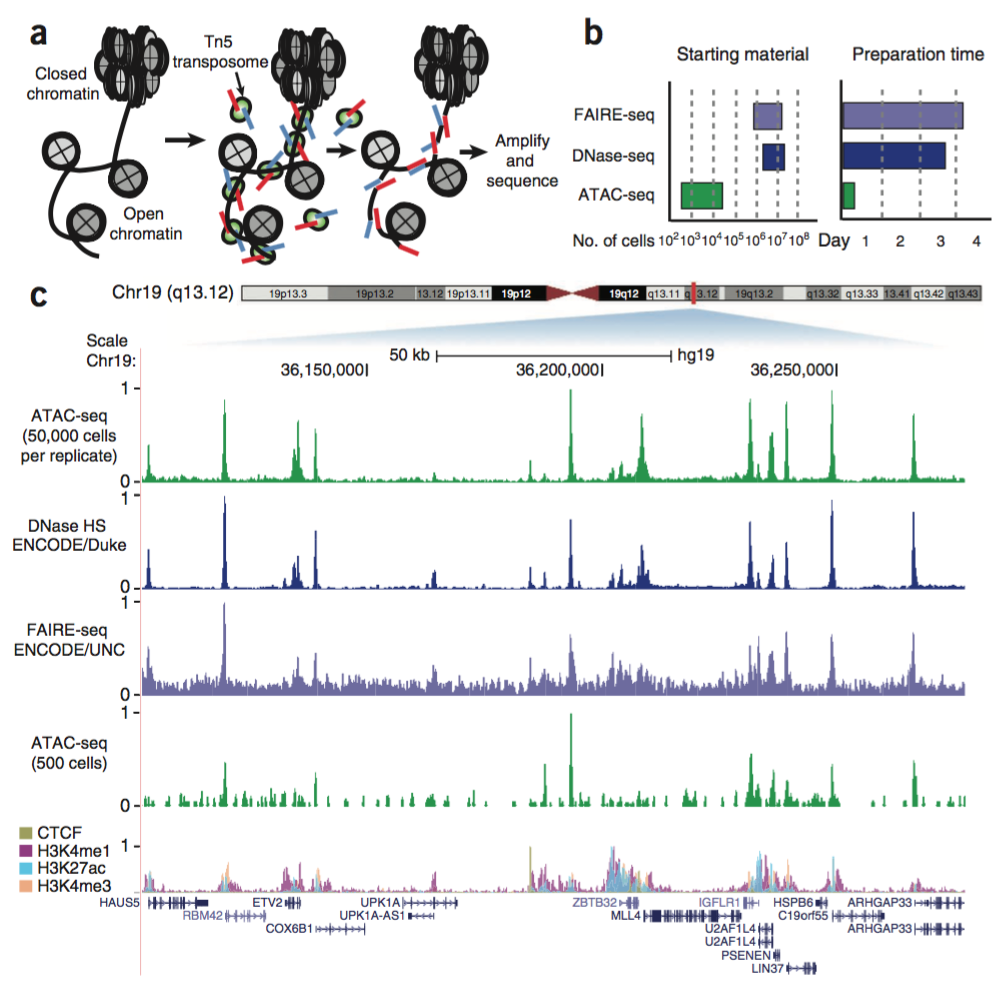
\includegraphics[height=0.85\paperheight]{whoiswho2.png}}
\end{frame}

\begin{frame}{ATAC-Seq length distribution}
\centering{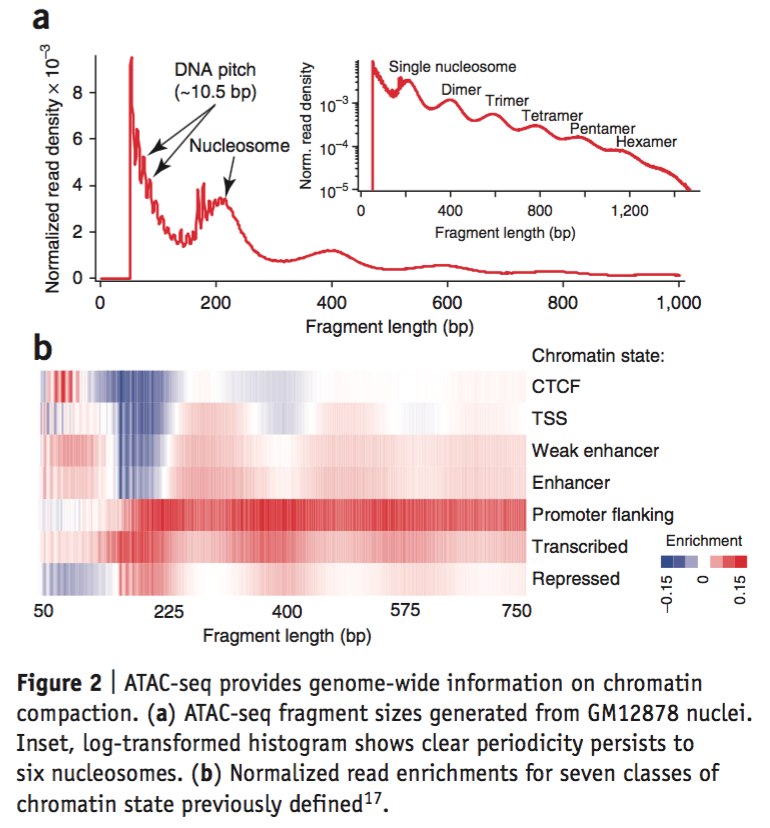
\includegraphics[height=0.85\paperheight]{length.png}}
\end{frame}

\begin{frame}{Summary}
Experimental:
\begin{itemize}
\item Peak intensities highly reproducible between technical replicates (R = 0.98) and DNase-seq data (R = 0.79 and R = 0.83)
\item Sensitivity was \textbf{diminished} for small $\leq 500$ numbers of input material.
\end{itemize}
Protocol:
\begin{itemize}
\item Relatively simple protocol that can be carried out in hours for a standard sample size of 50000 cells.
\item The \textbf{biggest} source of failure comes from variations in cell number.\footnote{Too few cells causes over-digestion of chromatin - reads that map to inaccessible regions (noise);\\too many cells causes under-digestion and creates high-molecular-weight fragments.}
\item For nucleosome mapping, paired-end sequencing is preferred.
\item Difference in human open chromatin human $\geq$ 50mln mapped reads
\item TF foot-printing $\geq$200mln mapped reads.
\item Half of reads are approximately of subnucleosomal length (150 bp) and half of the reads are longer.
\end{itemize}
\end{frame}


\begin{frame}{VS others}
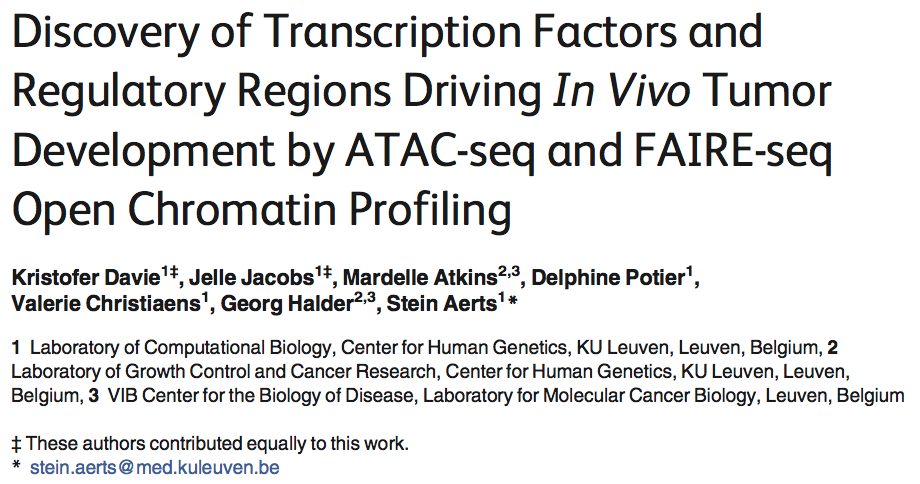
\includegraphics[width=\linewidth]{atac_vs_faire.png}\\
\tiny{Here we ask whether open chromatin profiling can be used to identify the entire repertoire of active promoters and enhancers underlying tissue-specific gene expression during normal development and onco- genesis in vivo.\\
In conclusion, we show that FAIRE-seq and ATAC-seq based open chromatin profiling, combined with motif discovery, is a straightforward approach to identify functional genomic regulatory regions, master regulators, and gene regulatory networks controlling complex in vivo processes.}
\end{frame}

\begin{frame}{Conclusions}
\begin{itemize}
\item Both methods are robust in identifying accessible or open regions.
\item ATAC-seq shows slightly lower background levels.
\item ATAC-seq shows a higher recall of true enhancers than FAIRE-seq.
\item ATAC can detect both smaller and greater significant differences between normal and tumor states than FAIRE.
\end{itemize}
\end{frame}


\begin{frame}{NucleoATAC\footnote{\url{https://github.com/GreenleafLab/NucleoATAC}}}
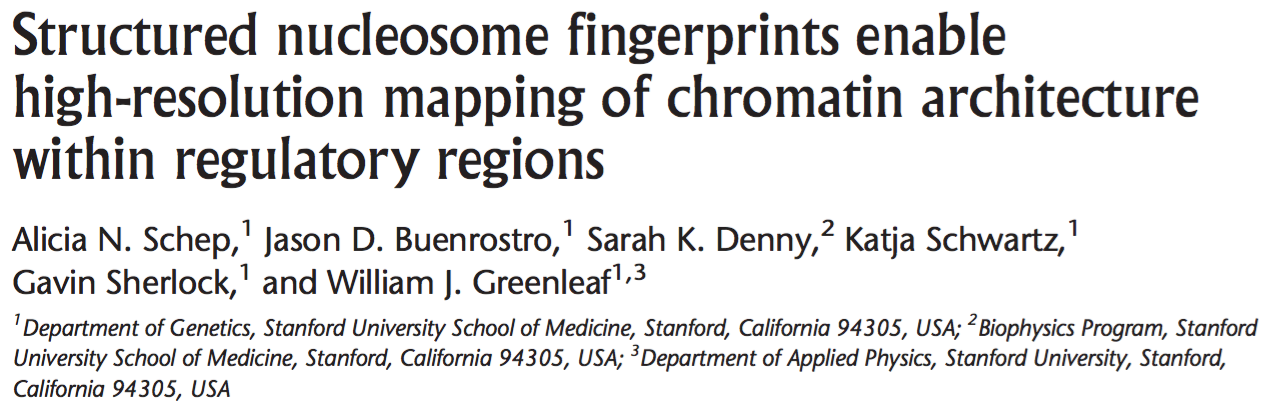
\includegraphics[width=\linewidth]{nucleoatac_paper.png}\\
\end{frame}

\begin{frame}{Existing tools}
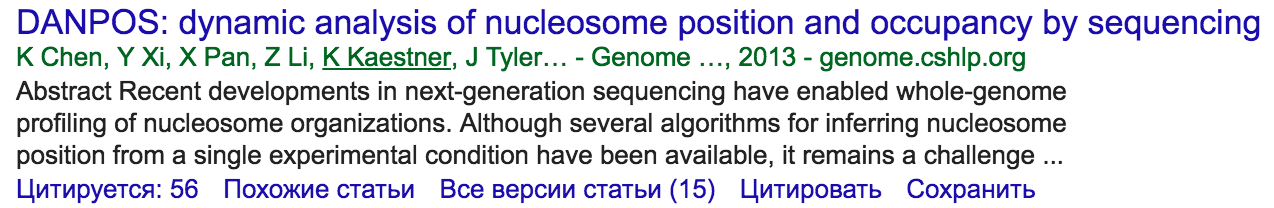
\includegraphics[height=0.20\paperheight]{Danpos.png}\\
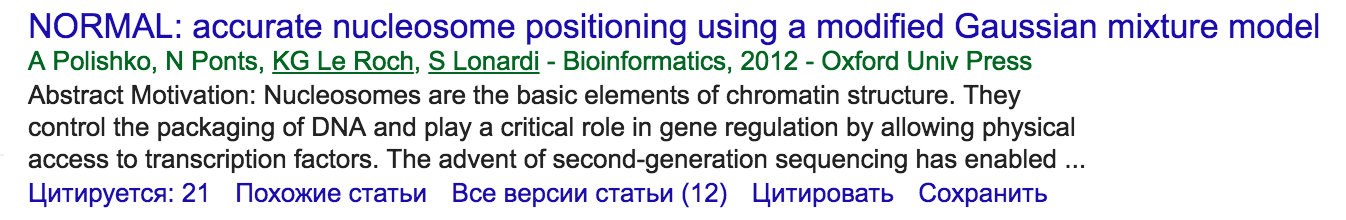
\includegraphics[height=0.20\paperheight]{Normal.png}\\\footnote{Based on gaussian mixtures.}
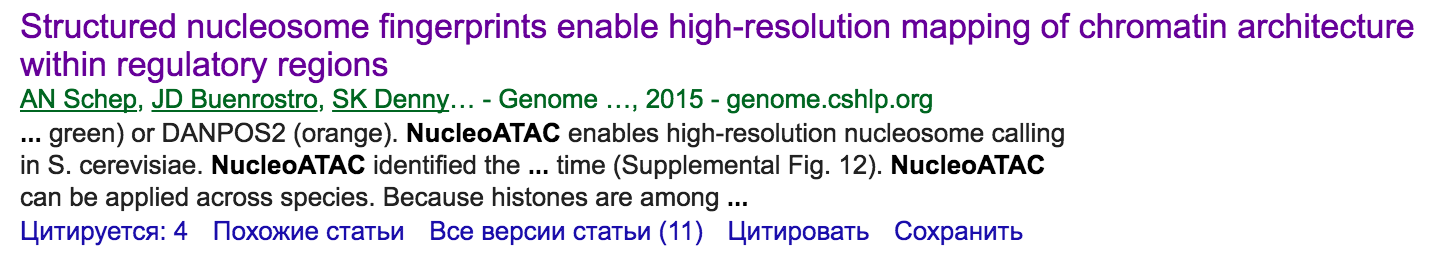
\includegraphics[height=0.20\paperheight]{nucleoatac.png}
\end{frame}

\begin{frame}
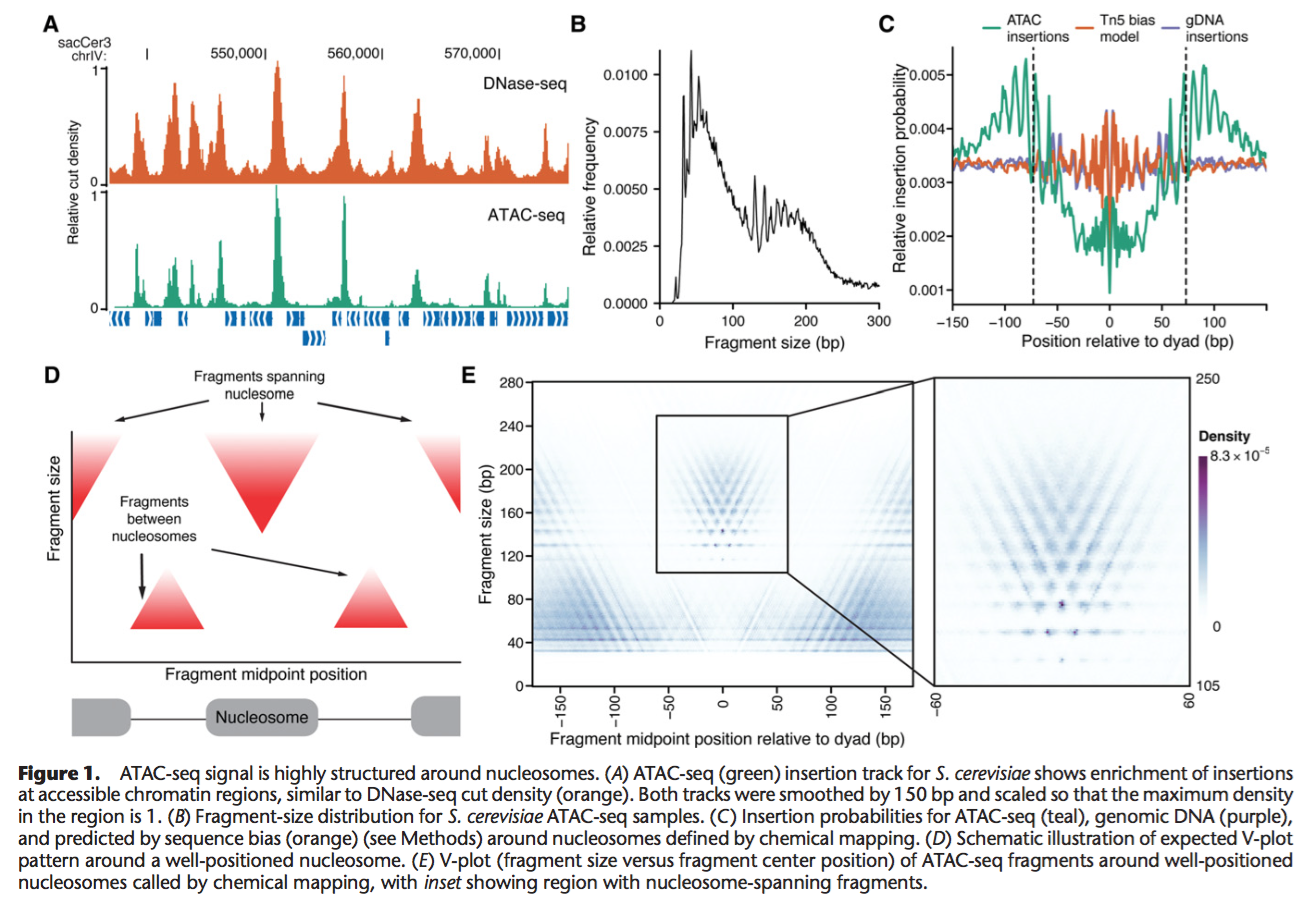
\includegraphics[width=\linewidth]{vshape.png}\\
\end{frame}

\begin{frame}{V-plot}
Density of fragment sizes versus fragment center locations relative to a genomic feature of interest.\footnote{Introduced in\url{http://www.cs.duke.edu/courses/compsci662/spring15/pdf/henikoff.2011.pdf}}
\begin{itemize}
\item Apex of the “V” represents the smallest possible fragment that spans the DNA protected by a nucleosome (117bp).
\item Horizontal and vertical periodicity likely reflects both the steric hindrance of the transposase (vertical and horizontal periodicity) and 10-bp rotational positioning of nucleosomes in \textit{yeast}. 
\item Stochastic “breathing” of DNA - most abundant position in the V-plot represents fragments of 143 bp centered at the dyad.
\item NucleoATAC identified the positions of 13344 nucleosomes across broad open chromatin regions in the yeast\footnote{ Z-score$\geq$3, log-likelihood ratio$\geq$ 0} out of 17015 chemical mapping.
\end{itemize}
\end{frame}

\begin{frame}{NucleoATAC vs DANPOS2}
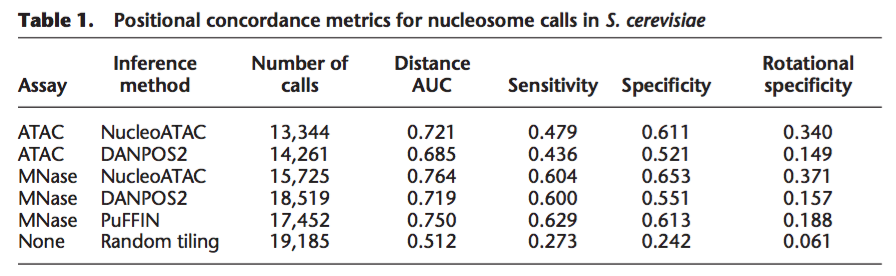
\includegraphics[width=\linewidth]{nucleoatac_danpose.png}\\
\end{frame}

\begin{frame}{Summary}
\begin{itemize}
\item Reads QC - ChiLin
\item Nucleosome positioning - NucleoATAC
\end{itemize}
\end{frame}

\begin{frame}
\centering{
	\Huge{\textit{Fin}}
}
%\vspace{10mm}
\end{frame}

\end{document}
